% Section 7.4 -- E4: CPU vs GPU vs fp64 (P3)
% Numbers from results/E4_cluster/*/E4_timing.csv.
% This file also holds the E5 figure, so E4 and E5 share one figure page.

\subsection{E4: Backend scaling (RQ4)}
\label{sec:e4}

E4 fixes the circuit at $p = 3$ and changes only the target.
Runs stop after different numbers of evaluations, so we compare time per evaluation.
Two settings hit the 24-hour limit, leaving one of three instances for GPU fp64 at $n = 30$ and two of three for the CPU at $n = 20$.

\begin{figure}[p]
  \centering
  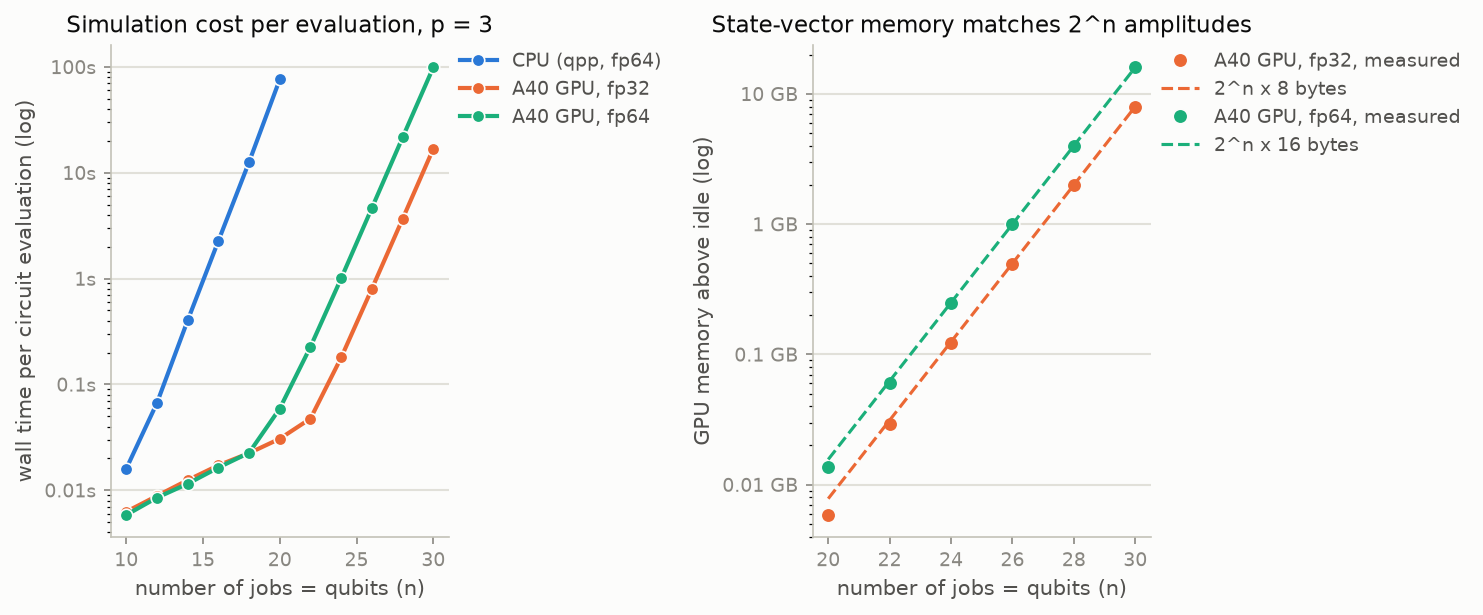
\includegraphics[width=\linewidth]{E4_timing.png}
  \caption{E4 at $p = 3$. Left: wall time per circuit evaluation (log scale). Right: GPU memory above an idle CUDA context against the $2^n$-amplitude prediction.}
  \label{fig:e4}
  \vspace{18pt}
  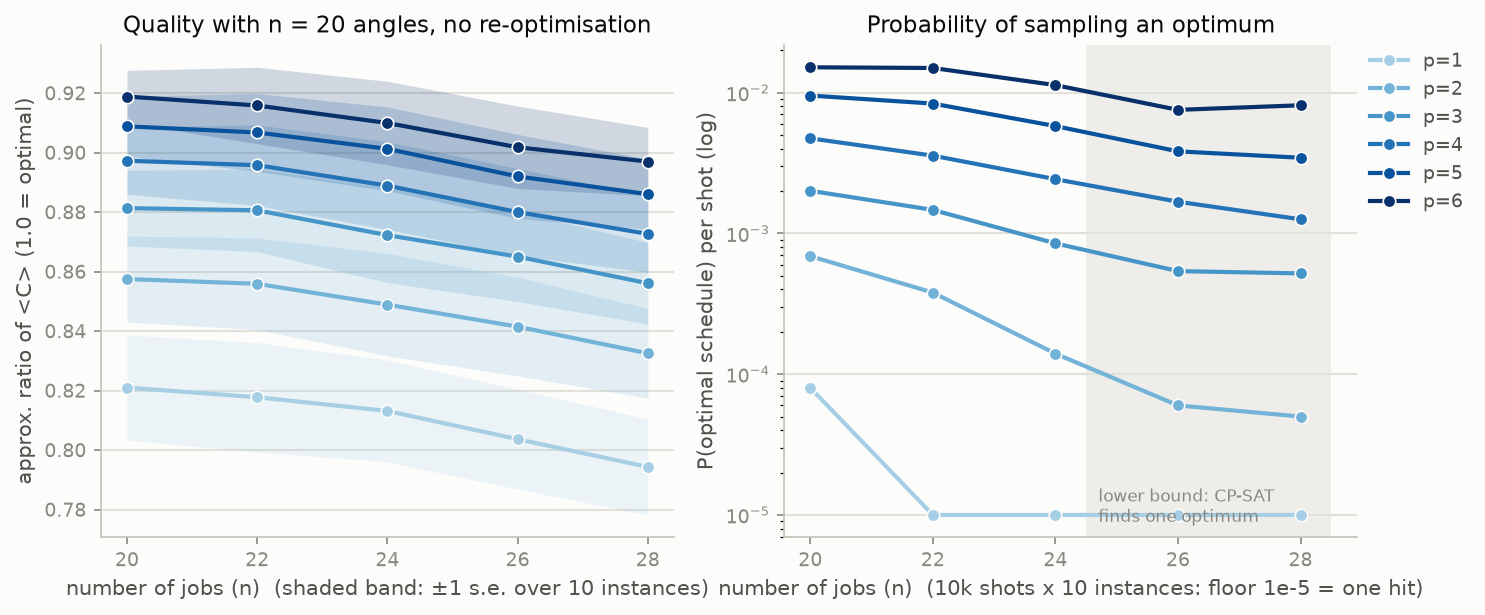
\includegraphics[width=\linewidth]{E5_largen.png}
  \caption{E5. Angles optimised at $n = 20$, reused without optimisation at $n = 20$--$28$. Left: approximation ratio by depth. Right: $P(\text{opt})$ (log scale), a lower bound above $n = 24$.}
  \label{fig:e5}
\end{figure}

At $n = 20$ the CPU takes $76$\,s and the GPU $31$\,ms, about $2{,}500$ times faster (Fig.~\ref{fig:e4}, left).
Each extra qubit doubles the amplitudes and the gate count also grows with $n$, so the CPU's cost grows five- to six-fold every two qubits, while the GPU stays nearly flat until about $n = 22$, where the work starts to fill it.
fp32 and fp64 cost about the same on the GPU up to $n = 18$, but fp64 is $1.9\times$ slower at $n = 20$ and $5.8$--$5.9\times$ slower from $n = 26$.
That is more than the $2\times$ of memory traffic alone, as the A40 has much lower fp64 throughput.
Measured GPU memory matches $2^n$ amplitudes at 8 or 16 bytes within 2\,\% from $n = 24$ (Fig.~\ref{fig:e4}, right), so one 48\,GB A40 holds at most 32 qubits in fp32 and 31 in fp64.
